\documentclass[a4paper,11pt]{article}
\usepackage[utf8]{inputenc}\usepackage[T1]{fontenc}
\usepackage[english]{babel}\usepackage{lmodern}\usepackage{microtype}
\usepackage{amsmath,amssymb}\usepackage{geometry}
\geometry{a4paper,left=2.2cm,right=2.2cm,top=2.0cm,bottom=2.0cm}
\usepackage{booktabs,array}\usepackage{xcolor}
\definecolor{bokug}{RGB}{0,135,60}\usepackage{tikz}
\usetikzlibrary{arrows.meta,calc}
\usepackage{fancyhdr}\pagestyle{fancy}
\renewcommand{\headrulewidth}{0.4pt}
\usepackage{enumitem}\setlength{\parindent}{0pt}\setlength{\parskip}{4pt}

\begin{document}
\fancyhead[L]{\small VU Mechanik – LAWI 100515 (PI)}\fancyhead[R]{\small SS 2026}\fancyfoot[C]{\thepage}
\begin{center}{\large\bfseries\color{bokug}University of Natural Resources and Life Sciences, Vienna (BOKU)}\\[2pt]{\large\bfseries VU Mechanik – LAWI 100515 (PI)}\\[4pt]Exam \textbf{Group A} \hfill Date: 26.06.2026\\[2pt]\rule{\linewidth}{0.4pt}\end{center}

\begin{center}\textbf{\large Model solution}\end{center}
\begin{center}
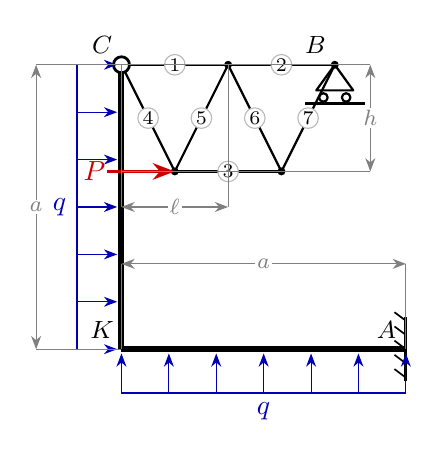
\begin{tikzpicture}[scale=0.903,>=Stealth,line join=round]
  \coordinate (P0) at (0.000,0.000);
  \coordinate (K) at (-4.000,0.000);
  \coordinate (C) at (-4.000,4.000);
  \coordinate (TO1) at (-2.500,4.000);
  \coordinate (TO2) at (-1.000,4.000);
  \coordinate (TU0) at (-3.250,2.500);
  \coordinate (TU1) at (-1.750,2.500);
  \draw[thick] (C) -- (TO1);
  \draw[thick] (TO1) -- (TO2);
  \draw[thick] (TU0) -- (TU1);
  \draw[thick] (C) -- (TU0);
  \draw[thick] (TU0) -- (TO1);
  \draw[thick] (TO1) -- (TU1);
  \draw[thick] (TU1) -- (TO2);
  \draw[line width=2.2pt] (P0) -- (K);
  \draw[line width=2.2pt] (K) -- (C);
  \fill (TO1) circle (1.6pt);
  \fill (TO2) circle (1.6pt);
  \fill (TU0) circle (1.6pt);
  \fill (TU1) circle (1.6pt);
  \draw[fill=white,line width=1pt] (C) circle (3.2pt);
  \draw[line width=1.1pt] (0.000,0.450) -- (0.000,-0.450);
  \draw[line width=0.6pt] (0.000,0.400) -- (-0.160,0.520);
  \draw[line width=0.6pt] (0.000,0.200) -- (-0.160,0.320);
  \draw[line width=0.6pt] (0.000,0.000) -- (-0.160,0.120);
  \draw[line width=0.6pt] (0.000,-0.200) -- (-0.160,-0.080);
  \draw[line width=0.6pt] (0.000,-0.400) -- (-0.160,-0.280);
  \draw[thick] (-1.000,4.000) -- (-1.260,3.640) -- (-0.740,3.640) -- cycle;
  \draw[thick] (-1.160,3.540) circle (0.06) (-0.840,3.540) circle (0.06);
  \draw[line width=1pt] (-1.420,3.460) -- (-0.580,3.460);
  \node[circle,fill=white,draw=gray!55,inner sep=0.5pt,font=\scriptsize] at (-3.250,4.000) {1};
  \node[circle,fill=white,draw=gray!55,inner sep=0.5pt,font=\scriptsize] at (-1.750,4.000) {2};
  \node[circle,fill=white,draw=gray!55,inner sep=0.5pt,font=\scriptsize] at (-2.500,2.500) {3};
  \node[circle,fill=white,draw=gray!55,inner sep=0.5pt,font=\scriptsize] at (-3.625,3.250) {4};
  \node[circle,fill=white,draw=gray!55,inner sep=0.5pt,font=\scriptsize] at (-2.875,3.250) {5};
  \node[circle,fill=white,draw=gray!55,inner sep=0.5pt,font=\scriptsize] at (-2.125,3.250) {6};
  \node[circle,fill=white,draw=gray!55,inner sep=0.5pt,font=\scriptsize] at (-1.375,3.250) {7};
  \draw[->,blue!70!black] (0.000,-0.620) -- (0.000,-0.060);
  \draw[->,blue!70!black] (-0.667,-0.620) -- (-0.667,-0.060);
  \draw[->,blue!70!black] (-1.333,-0.620) -- (-1.333,-0.060);
  \draw[->,blue!70!black] (-2.000,-0.620) -- (-2.000,-0.060);
  \draw[->,blue!70!black] (-2.667,-0.620) -- (-2.667,-0.060);
  \draw[->,blue!70!black] (-3.333,-0.620) -- (-3.333,-0.060);
  \draw[->,blue!70!black] (-4.000,-0.620) -- (-4.000,-0.060);
  \draw[blue!70!black,thick] (0.000,-0.620) -- (-4.000,-0.620);
  \node[blue!70!black] at (-2.000,-0.870) {$q$};
  \draw[->,blue!70!black] (-4.620,0.000) -- (-4.060,0.000);
  \draw[->,blue!70!black] (-4.620,0.667) -- (-4.060,0.667);
  \draw[->,blue!70!black] (-4.620,1.333) -- (-4.060,1.333);
  \draw[->,blue!70!black] (-4.620,2.000) -- (-4.060,2.000);
  \draw[->,blue!70!black] (-4.620,2.667) -- (-4.060,2.667);
  \draw[->,blue!70!black] (-4.620,3.333) -- (-4.060,3.333);
  \draw[->,blue!70!black] (-4.620,4.000) -- (-4.060,4.000);
  \draw[blue!70!black,thick] (-4.620,0.000) -- (-4.620,4.000);
  \node[blue!70!black] at (-4.870,2.000) {$q$};
  \draw[->,red!80!black,line width=1.1pt] (-4.200,2.500) -- (-3.250,2.500);
  \node[red!80!black] at (-4.380,2.500) {$P$};
  \draw[thin,gray] (0.000,0.000) -- (0.000,1.200);
  \draw[thin,gray] (-4.000,0.000) -- (-4.000,1.200);
  \draw[<->,gray] (0.000,1.200) -- (-4.000,1.200) node[midway,fill=white,inner sep=0.8pt,font=\footnotesize]{$a$};
  \draw[thin,gray] (-4.000,0.000) -- (-5.200,0.000);
  \draw[thin,gray] (-4.000,4.000) -- (-5.200,4.000);
  \draw[<->,gray] (-5.200,0.000) -- (-5.200,4.000) node[midway,fill=white,inner sep=0.8pt,font=\footnotesize]{$a$};
  \draw[thin,gray] (-4.000,4.000) -- (-4.000,2.000);
  \draw[thin,gray] (-2.500,4.000) -- (-2.500,2.000);
  \draw[<->,gray] (-4.000,2.000) -- (-2.500,2.000) node[midway,fill=white,inner sep=0.8pt,font=\footnotesize]{$\ell$};
  \draw[thin,gray] (-4.000,4.000) -- (-0.500,4.000);
  \draw[thin,gray] (-4.000,2.500) -- (-0.500,2.500);
  \draw[<->,gray] (-0.500,4.000) -- (-0.500,2.500) node[midway,fill=white,inner sep=0.8pt,font=\footnotesize]{$h$};
  \node[font=\small] at (0.000,0.000) [xshift=-7pt,yshift=7pt] {$A$};
  \node[font=\small] at (-4.000,0.000) [xshift=-7pt,yshift=7pt] {$K$};
  \node[font=\small] at (-4.000,4.000) [xshift=-7pt,yshift=7pt] {$C$};
  \node[font=\small] at (-1.000,4.000) [xshift=-7pt,yshift=7pt] {$B$};
\end{tikzpicture}
\end{center}
\par\medskip\textbf{1.\ Static determinacy}\par Counting criterion $n=3k-(a+z)$ (bodies $k$, reactions $a$, interaction forces $z$):
\[ n=3k-(a+z)=3\cdot2-(4+2)=0\ \Rightarrow\ \text{statically determinate} \]
\par\medskip\textbf{2.\ Support reactions and hinge forces}\par
$A:\ R_x=-24,\ R_y=-6,\ M=72$\quad $B:\ R_x=0,\ R_y=-6$\par $C:\ H_x=12,\ H_y=-6$
\par\medskip\textbf{3.\ Truss member forces}\par
\begin{center}\renewcommand{\arraystretch}{1.1}\begin{tabular}{c r l}
\toprule
Member & Force $S$ [kN] & Type \\
\midrule
  1 & 9 & tension \\
  2 & 3 & tension \\
  3 & -6 & compression \\
  4 & 6.71 & tension \\
  5 & -6.71 & compression \\
  6 & 6.71 & tension \\
  7 & -6.71 & compression \\
\bottomrule
\end{tabular}\end{center}
\begin{center}
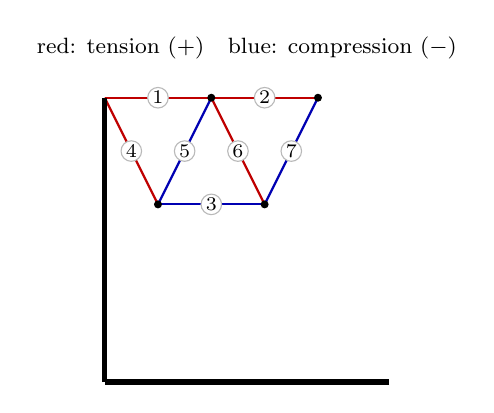
\begin{tikzpicture}[scale=0.903,>=Stealth,line join=round]
  \coordinate (P0) at (0.000,0.000);
  \coordinate (K) at (-4.000,0.000);
  \coordinate (C) at (-4.000,4.000);
  \coordinate (TO1) at (-2.500,4.000);
  \coordinate (TO2) at (-1.000,4.000);
  \coordinate (TU0) at (-3.250,2.500);
  \coordinate (TU1) at (-1.750,2.500);
  \draw[thick,red!75!black] (C) -- (TO1);
  \draw[thick,red!75!black] (TO1) -- (TO2);
  \draw[thick,blue!70!black] (TU0) -- (TU1);
  \draw[thick,red!75!black] (C) -- (TU0);
  \draw[thick,blue!70!black] (TU0) -- (TO1);
  \draw[thick,red!75!black] (TO1) -- (TU1);
  \draw[thick,blue!70!black] (TU1) -- (TO2);
  \draw[line width=2pt] (P0) -- (K);
  \draw[line width=2pt] (K) -- (C);
  \fill (TO1) circle (1.6pt);
  \fill (TO2) circle (1.6pt);
  \fill (TU0) circle (1.6pt);
  \fill (TU1) circle (1.6pt);
  \node[circle,fill=white,draw=gray!55,inner sep=0.5pt,font=\scriptsize] at (-3.250,4.000) {1};
  \node[circle,fill=white,draw=gray!55,inner sep=0.5pt,font=\scriptsize] at (-1.750,4.000) {2};
  \node[circle,fill=white,draw=gray!55,inner sep=0.5pt,font=\scriptsize] at (-2.500,2.500) {3};
  \node[circle,fill=white,draw=gray!55,inner sep=0.5pt,font=\scriptsize] at (-3.625,3.250) {4};
  \node[circle,fill=white,draw=gray!55,inner sep=0.5pt,font=\scriptsize] at (-2.875,3.250) {5};
  \node[circle,fill=white,draw=gray!55,inner sep=0.5pt,font=\scriptsize] at (-2.125,3.250) {6};
  \node[circle,fill=white,draw=gray!55,inner sep=0.5pt,font=\scriptsize] at (-1.375,3.250) {7};
  \node[font=\footnotesize] at (-2.00,4.70) {red: tension $(+)$\quad blue: compression $(-)$};
\end{tikzpicture}
\end{center}
\par\medskip\textbf{4.\ Section-force diagrams of the beams}\par
\begin{center}
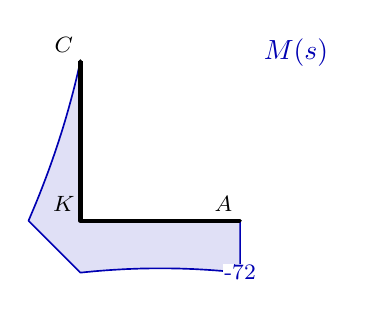
\begin{tikzpicture}[scale=0.507,line join=round]
  \filldraw[fill=blue!70!black!12,draw=blue!70!black,semithick] (0.000,-1.300) -- (-0.167,-1.283) -- (-0.333,-1.267) -- (-0.500,-1.253) -- (-0.667,-1.240) -- (-0.833,-1.229) -- (-1.000,-1.219) -- (-1.167,-1.210) -- (-1.333,-1.204) -- (-1.500,-1.198) -- (-1.667,-1.195) -- (-1.833,-1.192) -- (-2.000,-1.192) -- (-2.167,-1.192) -- (-2.333,-1.195) -- (-2.500,-1.198) -- (-2.667,-1.204) -- (-2.833,-1.210) -- (-3.000,-1.219) -- (-3.167,-1.229) -- (-3.333,-1.240) -- (-3.500,-1.253) -- (-3.667,-1.267) -- (-3.833,-1.283) -- (-4.000,-1.300) -- (-5.300,0.000) -- (-5.229,0.167) -- (-5.159,0.333) -- (-5.090,0.500) -- (-5.023,0.667) -- (-4.958,0.833) -- (-4.894,1.000) -- (-4.831,1.167) -- (-4.770,1.333) -- (-4.711,1.500) -- (-4.653,1.667) -- (-4.597,1.833) -- (-4.542,2.000) -- (-4.488,2.167) -- (-4.436,2.333) -- (-4.386,2.500) -- (-4.337,2.667) -- (-4.290,2.833) -- (-4.244,3.000) -- (-4.199,3.167) -- (-4.156,3.333) -- (-4.115,3.500) -- (-4.075,3.667) -- (-4.037,3.833) -- (-4.000,4.000) -- (-4.000,4.000) -- (-4.000,3.833) -- (-4.000,3.667) -- (-4.000,3.500) -- (-4.000,3.333) -- (-4.000,3.167) -- (-4.000,3.000) -- (-4.000,2.833) -- (-4.000,2.667) -- (-4.000,2.500) -- (-4.000,2.333) -- (-4.000,2.167) -- (-4.000,2.000) -- (-4.000,1.833) -- (-4.000,1.667) -- (-4.000,1.500) -- (-4.000,1.333) -- (-4.000,1.167) -- (-4.000,1.000) -- (-4.000,0.833) -- (-4.000,0.667) -- (-4.000,0.500) -- (-4.000,0.333) -- (-4.000,0.167) -- (-4.000,0.000) -- (-4.000,0.000) -- (-3.833,0.000) -- (-3.667,0.000) -- (-3.500,0.000) -- (-3.333,0.000) -- (-3.167,0.000) -- (-3.000,0.000) -- (-2.833,0.000) -- (-2.667,0.000) -- (-2.500,0.000) -- (-2.333,0.000) -- (-2.167,0.000) -- (-2.000,0.000) -- (-1.833,0.000) -- (-1.667,0.000) -- (-1.500,0.000) -- (-1.333,0.000) -- (-1.167,0.000) -- (-1.000,0.000) -- (-0.833,0.000) -- (-0.667,0.000) -- (-0.500,0.000) -- (-0.333,0.000) -- (-0.167,0.000) -- (0.000,0.000) -- cycle;
  \draw[line width=1.6pt] (0.000,0.000) -- (-4.000,0.000) -- (-4.000,4.000);
  \node[blue!70!black,font=\footnotesize,fill=white,inner sep=0.5pt] at (0.000,-1.300) {-72};
  \fill (0.000,0.000) circle (1.3pt);
  \node[font=\footnotesize] at (0.000,0.000) [xshift=-6pt,yshift=6pt] {$A$};
  \fill (-4.000,0.000) circle (1.3pt);
  \node[font=\footnotesize] at (-4.000,0.000) [xshift=-6pt,yshift=6pt] {$K$};
  \fill (-4.000,4.000) circle (1.3pt);
  \node[font=\footnotesize] at (-4.000,4.000) [xshift=-6pt,yshift=6pt] {$C$};
  \node[blue!70!black,right] at (0.35,4.20) {$M(s)$};
\end{tikzpicture}\\[5pt]
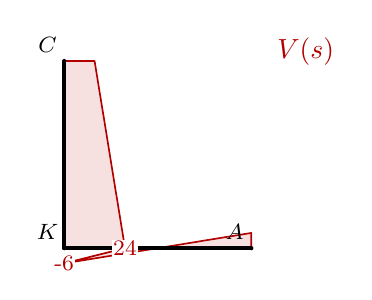
\begin{tikzpicture}[scale=0.594,line join=round]
  \filldraw[fill=red!70!black!12,draw=red!70!black,semithick] (0.000,0.325) -- (-0.167,0.298) -- (-0.333,0.271) -- (-0.500,0.244) -- (-0.667,0.217) -- (-0.833,0.190) -- (-1.000,0.163) -- (-1.167,0.135) -- (-1.333,0.108) -- (-1.500,0.081) -- (-1.667,0.054) -- (-1.833,0.027) -- (-2.000,0.000) -- (-2.167,-0.027) -- (-2.333,-0.054) -- (-2.500,-0.081) -- (-2.667,-0.108) -- (-2.833,-0.135) -- (-3.000,-0.163) -- (-3.167,-0.190) -- (-3.333,-0.217) -- (-3.500,-0.244) -- (-3.667,-0.271) -- (-3.833,-0.298) -- (-4.000,-0.325) -- (-2.700,0.000) -- (-2.727,0.167) -- (-2.754,0.333) -- (-2.781,0.500) -- (-2.808,0.667) -- (-2.835,0.833) -- (-2.862,1.000) -- (-2.890,1.167) -- (-2.917,1.333) -- (-2.944,1.500) -- (-2.971,1.667) -- (-2.998,1.833) -- (-3.025,2.000) -- (-3.052,2.167) -- (-3.079,2.333) -- (-3.106,2.500) -- (-3.133,2.667) -- (-3.160,2.833) -- (-3.188,3.000) -- (-3.215,3.167) -- (-3.242,3.333) -- (-3.269,3.500) -- (-3.296,3.667) -- (-3.323,3.833) -- (-3.350,4.000) -- (-4.000,4.000) -- (-4.000,3.833) -- (-4.000,3.667) -- (-4.000,3.500) -- (-4.000,3.333) -- (-4.000,3.167) -- (-4.000,3.000) -- (-4.000,2.833) -- (-4.000,2.667) -- (-4.000,2.500) -- (-4.000,2.333) -- (-4.000,2.167) -- (-4.000,2.000) -- (-4.000,1.833) -- (-4.000,1.667) -- (-4.000,1.500) -- (-4.000,1.333) -- (-4.000,1.167) -- (-4.000,1.000) -- (-4.000,0.833) -- (-4.000,0.667) -- (-4.000,0.500) -- (-4.000,0.333) -- (-4.000,0.167) -- (-4.000,0.000) -- (-4.000,0.000) -- (-3.833,0.000) -- (-3.667,0.000) -- (-3.500,0.000) -- (-3.333,0.000) -- (-3.167,0.000) -- (-3.000,0.000) -- (-2.833,0.000) -- (-2.667,0.000) -- (-2.500,0.000) -- (-2.333,0.000) -- (-2.167,0.000) -- (-2.000,0.000) -- (-1.833,0.000) -- (-1.667,0.000) -- (-1.500,0.000) -- (-1.333,0.000) -- (-1.167,0.000) -- (-1.000,0.000) -- (-0.833,0.000) -- (-0.667,0.000) -- (-0.500,0.000) -- (-0.333,0.000) -- (-0.167,0.000) -- (0.000,0.000) -- cycle;
  \draw[line width=1.6pt] (0.000,0.000) -- (-4.000,0.000) -- (-4.000,4.000);
  \node[red!70!black,font=\footnotesize,fill=white,inner sep=0.5pt] at (-4.000,-0.325) {-6};
  \node[red!70!black,font=\footnotesize,fill=white,inner sep=0.5pt] at (-2.700,0.000) {24};
  \fill (0.000,0.000) circle (1.3pt);
  \node[font=\footnotesize] at (0.000,0.000) [xshift=-6pt,yshift=6pt] {$A$};
  \fill (-4.000,0.000) circle (1.3pt);
  \node[font=\footnotesize] at (-4.000,0.000) [xshift=-6pt,yshift=6pt] {$K$};
  \fill (-4.000,4.000) circle (1.3pt);
  \node[font=\footnotesize] at (-4.000,4.000) [xshift=-6pt,yshift=6pt] {$C$};
  \node[red!70!black,right] at (0.35,4.20) {$V(s)$};
\end{tikzpicture}\\[5pt]
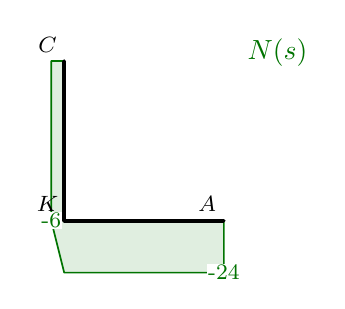
\begin{tikzpicture}[scale=0.507,line join=round]
  \filldraw[fill=green!45!black!12,draw=green!45!black,semithick] (0.000,-1.300) -- (-0.167,-1.300) -- (-0.333,-1.300) -- (-0.500,-1.300) -- (-0.667,-1.300) -- (-0.833,-1.300) -- (-1.000,-1.300) -- (-1.167,-1.300) -- (-1.333,-1.300) -- (-1.500,-1.300) -- (-1.667,-1.300) -- (-1.833,-1.300) -- (-2.000,-1.300) -- (-2.167,-1.300) -- (-2.333,-1.300) -- (-2.500,-1.300) -- (-2.667,-1.300) -- (-2.833,-1.300) -- (-3.000,-1.300) -- (-3.167,-1.300) -- (-3.333,-1.300) -- (-3.500,-1.300) -- (-3.667,-1.300) -- (-3.833,-1.300) -- (-4.000,-1.300) -- (-4.325,0.000) -- (-4.325,0.167) -- (-4.325,0.333) -- (-4.325,0.500) -- (-4.325,0.667) -- (-4.325,0.833) -- (-4.325,1.000) -- (-4.325,1.167) -- (-4.325,1.333) -- (-4.325,1.500) -- (-4.325,1.667) -- (-4.325,1.833) -- (-4.325,2.000) -- (-4.325,2.167) -- (-4.325,2.333) -- (-4.325,2.500) -- (-4.325,2.667) -- (-4.325,2.833) -- (-4.325,3.000) -- (-4.325,3.167) -- (-4.325,3.333) -- (-4.325,3.500) -- (-4.325,3.667) -- (-4.325,3.833) -- (-4.325,4.000) -- (-4.000,4.000) -- (-4.000,3.833) -- (-4.000,3.667) -- (-4.000,3.500) -- (-4.000,3.333) -- (-4.000,3.167) -- (-4.000,3.000) -- (-4.000,2.833) -- (-4.000,2.667) -- (-4.000,2.500) -- (-4.000,2.333) -- (-4.000,2.167) -- (-4.000,2.000) -- (-4.000,1.833) -- (-4.000,1.667) -- (-4.000,1.500) -- (-4.000,1.333) -- (-4.000,1.167) -- (-4.000,1.000) -- (-4.000,0.833) -- (-4.000,0.667) -- (-4.000,0.500) -- (-4.000,0.333) -- (-4.000,0.167) -- (-4.000,0.000) -- (-4.000,0.000) -- (-3.833,0.000) -- (-3.667,0.000) -- (-3.500,0.000) -- (-3.333,0.000) -- (-3.167,0.000) -- (-3.000,0.000) -- (-2.833,0.000) -- (-2.667,0.000) -- (-2.500,0.000) -- (-2.333,0.000) -- (-2.167,0.000) -- (-2.000,0.000) -- (-1.833,0.000) -- (-1.667,0.000) -- (-1.500,0.000) -- (-1.333,0.000) -- (-1.167,0.000) -- (-1.000,0.000) -- (-0.833,0.000) -- (-0.667,0.000) -- (-0.500,0.000) -- (-0.333,0.000) -- (-0.167,0.000) -- (0.000,0.000) -- cycle;
  \draw[line width=1.6pt] (0.000,0.000) -- (-4.000,0.000) -- (-4.000,4.000);
  \node[green!45!black,font=\footnotesize,fill=white,inner sep=0.5pt] at (0.000,-1.300) {-24};
  \node[green!45!black,font=\footnotesize,fill=white,inner sep=0.5pt] at (-4.325,0.000) {-6};
  \fill (0.000,0.000) circle (1.3pt);
  \node[font=\footnotesize] at (0.000,0.000) [xshift=-6pt,yshift=6pt] {$A$};
  \fill (-4.000,0.000) circle (1.3pt);
  \node[font=\footnotesize] at (-4.000,0.000) [xshift=-6pt,yshift=6pt] {$K$};
  \fill (-4.000,4.000) circle (1.3pt);
  \node[font=\footnotesize] at (-4.000,4.000) [xshift=-6pt,yshift=6pt] {$C$};
  \node[green!45!black,right] at (0.35,4.20) {$N(s)$};
\end{tikzpicture}\\[10pt]
\end{center}
\end{document}